\begin{figure}
\begin{leftfullpage}
\caption[Example of partial correlation structure]{
{\bf Example of partial correlation structure from $C_{\sf sparse+latent}$.}
{\bf A, B.} The regularized estimate $C_{\sf sparse+latent}$ closely approximates the sample correlation matrix $C_{\sf sample}$.
{\bf C, D.} The partial correlation matrices from the two estimates differ substantially.
{\bf E.} The partial correlation matrix of the regularized estimate is decomposed into a sparse component with 92.8\% off-diagonal zeros (bottom-left) and low-rank component of rank 72 (top-right).
{\bf F.} The sparse component of the regularized partial correlation matrix had little resemblance to the sample correlations: The gray region indicates the range of correlations containing 92.8\% of cells pairs, equal to the fraction of zeros in the sparse partial correlation matrix. Correlation coefficients outside this interval formed the network of greatest correlations.  This network differed from the sparse component of the $C_{\sf sparse+latent}$:  Only 27.7\% of the highest correlations coefficients outside the gray regions coincided with interactions inferred by $C_{\sf sparse+latent}$.
{\bf G.} A graphical depiction of the positive (green) and negative (magenta) sparse partial correlations as edges between observed neurons. The line density is proportional to the magnitude of the partial correlation.
{\bf H.} A subset of neurons from the center of the cluster shown in {\bf G} showing the sparse partial correlations.
{\bf I.} The same subset of neurons with edges indicating sample correlations thresholded to match the sparsity of the sparse partial correlation. These edges correspond to the sample correlation coefficients outside the gray region in panel F.
}\label{fig:4}
\end{leftfullpage}
\end{figure}

\begin{figure}
\begin{fullpage}
        \begin{center}
        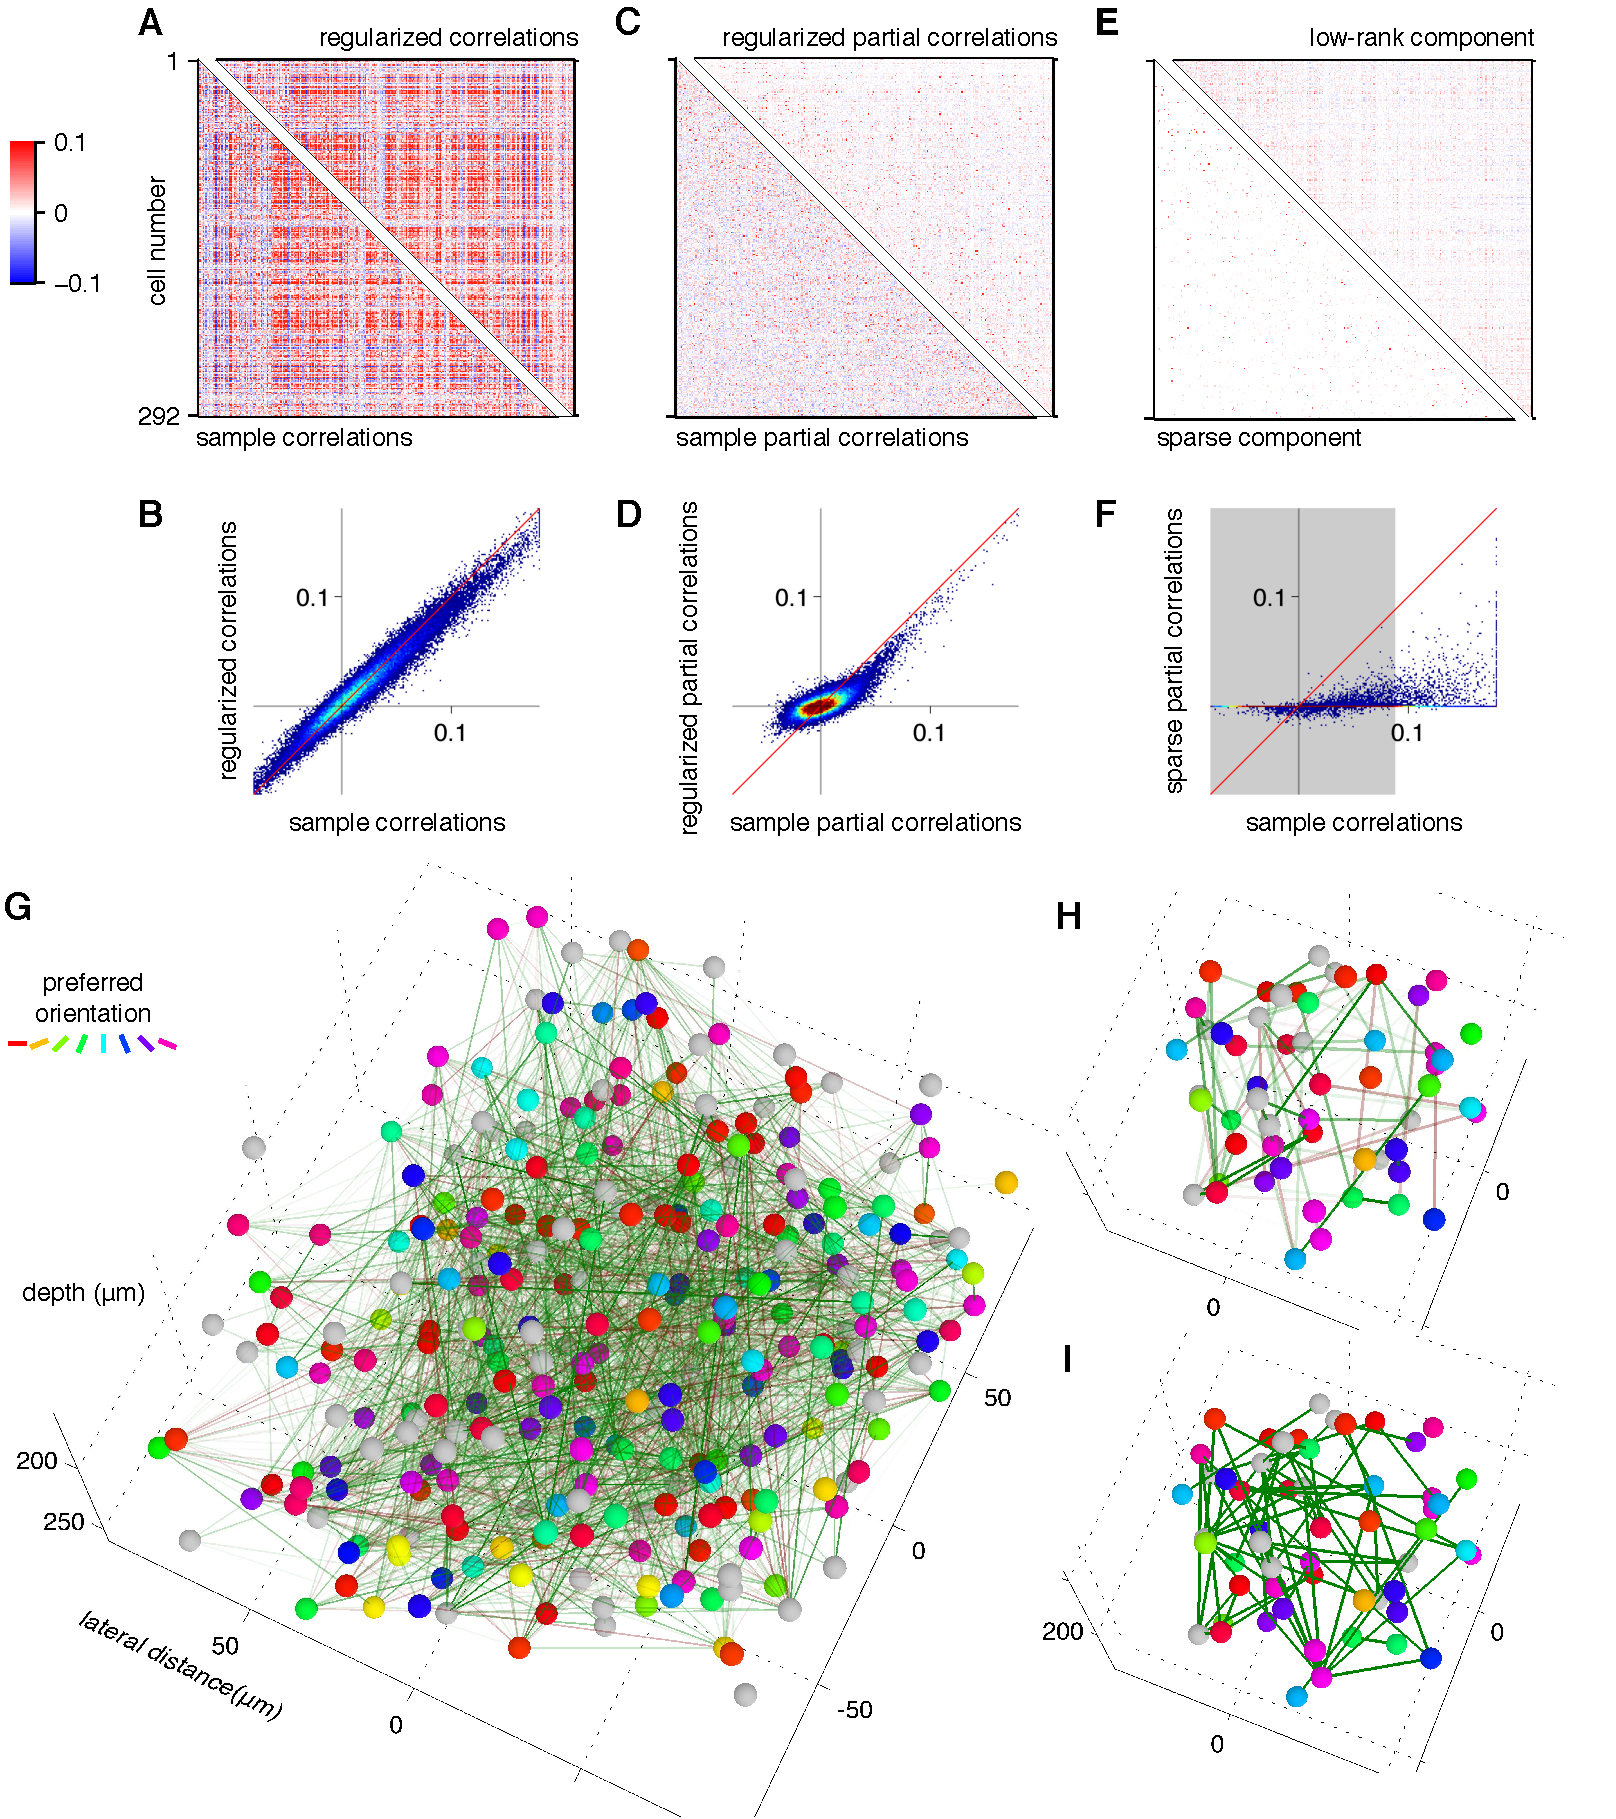
\includegraphics[height=\textwidth]{./figures/Reconstruction.pdf}
        \end{center}
\end{fullpage}
\end{figure}
